\renewcommand{\thechapter}{8}
\chapter{Conclusions and Future Plans}
\label{ch:Conclusions}

This work has presented a wide-ranging upgrade to the scintillation analysis of EXO-200.  The result has been an energy resolution and correspondingly lo waveform analysis techniques for scintillation energy measurements in EXO-200.  


\begin{figure}
\begin{center}
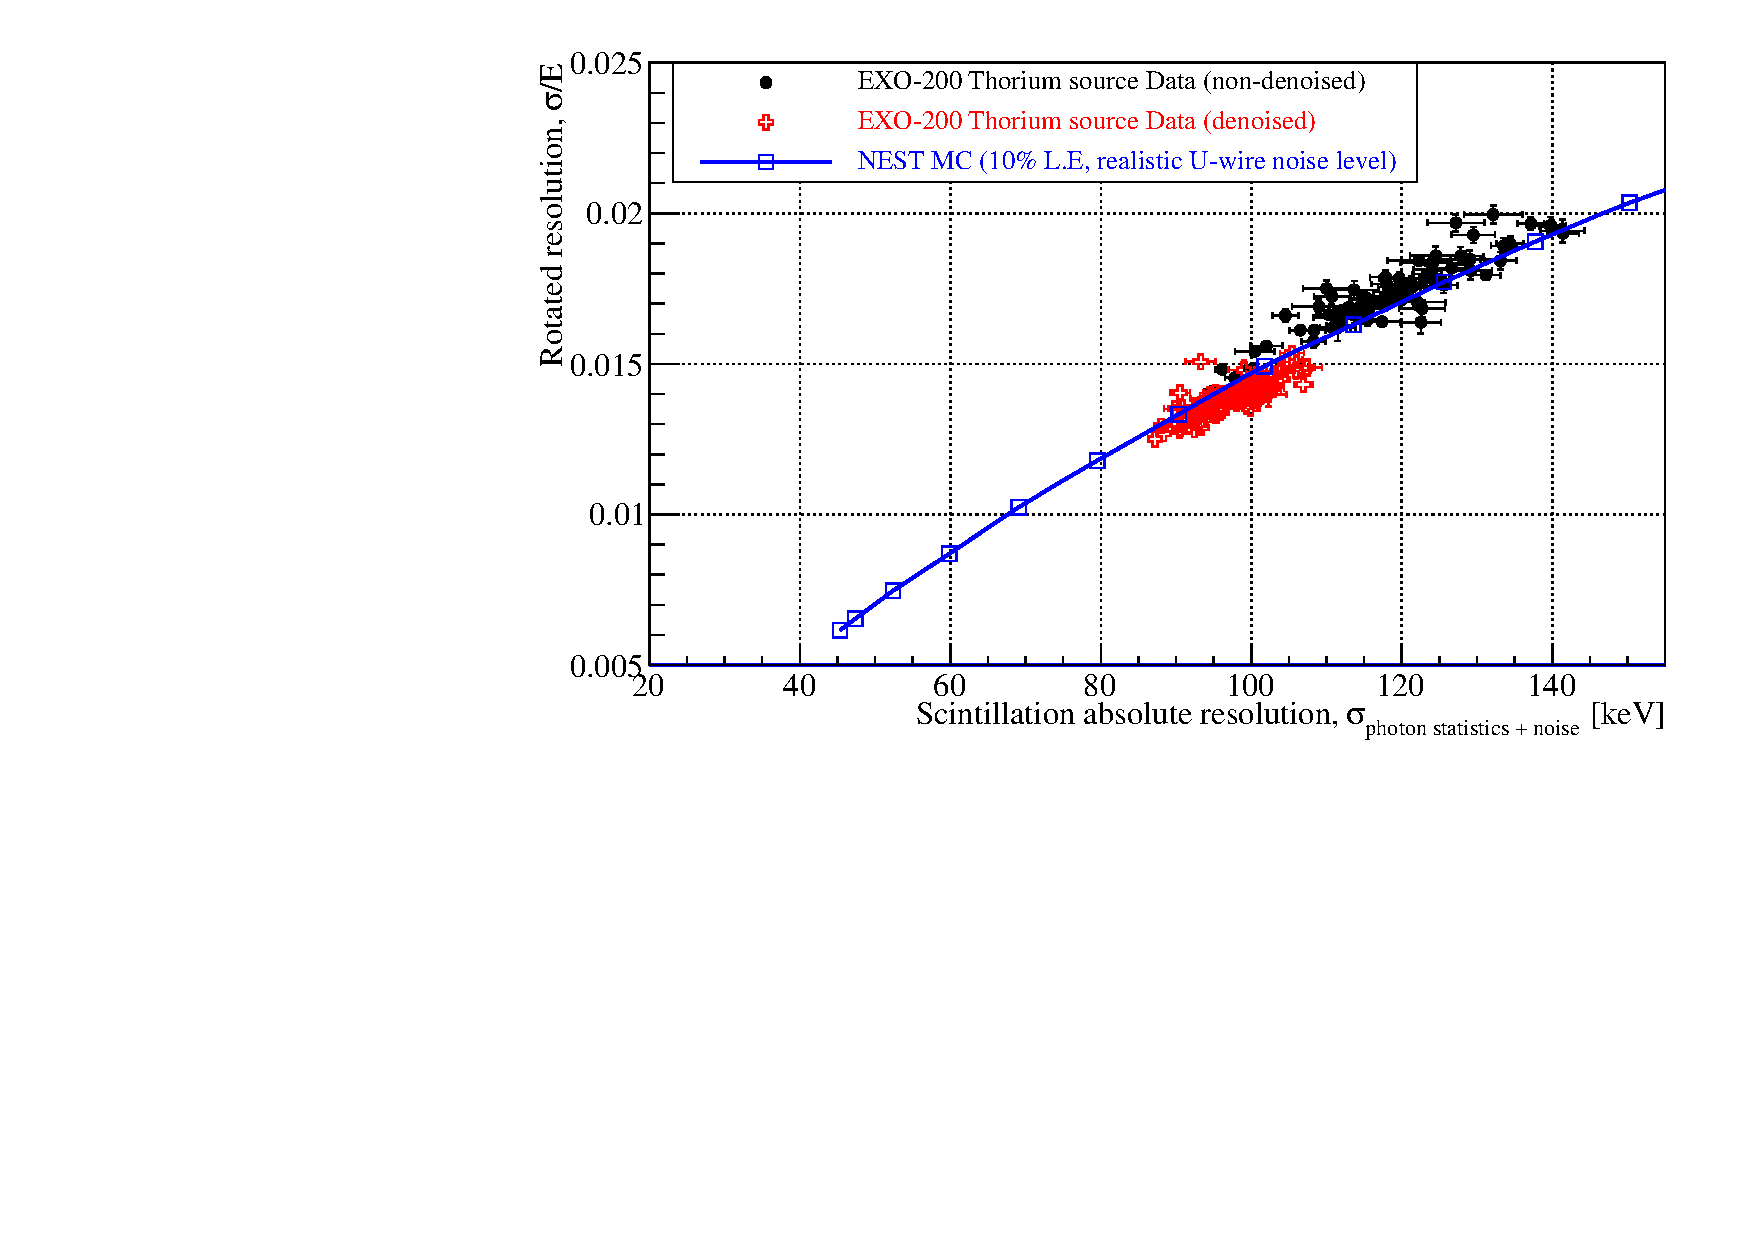
\includegraphics[keepaspectratio=true,width=\textwidth]{resoDataMC_800eRMSInIonization_Comp.pdf}
\end{center}
\renewcommand{\baselinestretch}{1}
\small\normalsize
\begin{quote}
\caption{NEST simulation software has been used to estimate how the rotated energy resolution at 2615 keV (vertical axis) depends on the scintillation-only resolution at 2615 keV (horizontal axis); this theoretical estimate is shown in blue, as applicable to the EXO-200 detector with fixed electric field and charge-only resolution.  Black points indicate measurements from thorium source runs without denoising; red points indicate measurements from thorium runs with denoising.  Figure provided by Liangjian Wen using NEST software~\cite{NESTpaper}.}
\label{fig:ScintillationVsOverallResolution_NEST}
\end{quote}
\end{figure}
\renewcommand{\baselinestretch}{2}
\small\normalsize

One question which must be asked is whether there is any room for further improvement in the energy resolution.  Figure~\ref{fig:ScintillationVsOverallResolution_NEST} shows simulations of the relationship between scintillation-only resolution and rotated energy resolution.  Points indicate the resolutions measured from denoised and non-denoised data; we can see that the model agrees well with both sets of data.  Based on these simulations, it is clear that further improvements to the scintillation resolution will indeed have a significant impact on the overall resolution of EXO-200; so further attempts to improve our resolution are indeed worthwhile.

We have already noted in section~\ref{sec:DenoisingInPractice} that the parameters used for this denoising were not optimal, and that preliminary studies indicate roughly 0.05 percentage points can be gained in overall energy resolution at 2615 keV by updating to an up-to-date set of denoising parameters.  This issue is straightforward to address, and the next processing of our dataset will incorporate it.

Beyond this improvement, we have described in section~\ref{sec:ResultEnergyLight} that the denoised scintillation peak position displays a large position dependence which cannot be fully calibrated in downstream analysis.  The effect of this feature is to dilute our resolution improvements.  Although the cause of this position dependence is not fully understood, we believe that it must originate in flaws in the lightmap because the lightmap is the input to denoising which encodes position-dependent yield information; one preliminary theory is that the discrepancy between 1-wire and 2-wire charge peak positions described in section~\ref{sec:ResultEnergyCharge} leads to a bias in event selection for the lightmap.  We believe that this will be an issue in denoising which can be addressed with further investigation and will lead to additional significant improvements in resolution.

The most exciting improvement in resolution may come not from offline analysis but from planned electronics upgrades.  There are indications that the source of electronic noise in the APDs is now understood and can be fixed in hardware in the near future, with an expectation of energy resolutions below 1\% after all upgrades~\cite{ElectronicsUpgradeReport_March2014}.  Energy resolution improvements on this scale would have a significant impact on backgrounds and the sensitivity of EXO-200 to $\beta\beta 0\nu$ decay.

One may wonder, after a hardware upgrade which reduces electronic noise on the APDs, whether denoising will still be a necessary component of the analysis.  It may indeed be the case that the full denoising scheme is not needed for lower-noise waveforms.  However, certain components of this analysis will still be critical to good resolution.  In particular, the techniques developed in this work to measure an APD-by-APD lightmap will still be needed to keep the energy resolution due to mismeasured gains low; we have seen hints in section~\ref{sec:ResultComparisonEnergy} that denoising has reduced the impact of gain mismatch by a factor of 9.7 in single-site data, and if true then this will be a critical component of any scintillation measurements regardless of changes in electronic noise.


Future plans to mention:
\begin{itemize}
\item Run1 contains up to 90 livetime-days, which is not negligible; denoising should have a significant improvement in resolution to offer even though APD gains were lower then.  (Personal view -- our next paper should include a combined analysis of Run1+Run2abcde.)
\item Further improvements in denoising are known to be acheivable.
\item Electronics upgrade could be a future hardware improvement.
\item Restate some of the things listed in denoising, like anticorrelated cluster energies.
\item denoised u-wires for improved risetime.
\item lower threshold in scintillation.
\item understand how gain non-uniformity plays into resolution, and implications for nEXO.
\end{itemize}
